\chapter{METODOLOGÍA}
Las metodologías de software ordenan y promueven buenas prácticas en el desarrollo de software de calidad, actualmente se encuentran numerosos modelos y metodologías que se pueden adaptar dependiendo las necesidades del producto final a entregar\parencite{Nohemy2015ESCOGERDECISION}. Para el proyecto “NOMBRE DEL PROYECTO” se identificaron dos perspectivas importantes que orientan la selección de la metodología, inicialmente debe permitir el desarrollo en un marco de tiempo corto; para este proyecto en específico de 6 meses y por otra parte necesita una verificación diaria con participación constante de expertos, permitiendo un crecimiento preciso y controlado, en donde se tomen decisiones rápidas y adaptables acorde al desarrollo de la aplicación.


Antes de comenzar es necesario definir el producto, el equipo de SCRUM y las tareas generales a realizar, para así elaborar la estructura del proyecto con la metodología, el equipo de trabajo estará compuesto así: 
\begin{itemize}
    \item Product Owner:  Con el objetivo de tener varios puntos de vista, hemos conseguido un grupo de profesionales que nos permiten tener una visión interdisciplinar para cumplirán este rol.
    \begin{enumerate}
        \item Diana Rivera Castillo, Ingeniera industrial con especialización en salud ocupacional, Youtuber Colombiana más influyente en Salud y seguridad en el trabajo SST, y actual Gerente de HSEQ Nueva Visión.
        \item Jorge Enrique Moreno Collazos, Fisioterapeuta, especialista en rehabilitación Cardiopulmonar, magíster en ciencias de la actividad física y el deporte, magíster en calidad educativa, doctor en salud pública, doctor en terapia manual, doctor en educación, Pos doctorado en educación, ciencias sociales e interculturalidad. Docente e investigador.
        \item Ximena Cano, Médica de la Universidad de Ciencias Aplicadas y Ambientales U.D.C.A. 
    \end{enumerate}

\item Scrum Master: esté cargo estará ocupado por Daniel Nieto Gomez.
\item Equipo desarrollador: Estará compuesto por Junior Parra como desarrollador de Scripting en Back end C\# y análisis de software, junto con Daniel Nieto Gómez como diseñador y desarrollador Front end y Análisis enfocado en el uso de herramientas de IA (inteligencia artificial). 
\end{itemize}

La duración del Sprint será de semana y media, por el periodo correspondiente al proyecto, es decir, 6 meses.

Por tratarse de un producto de software, la primera tarea a llevar a cabo es la ingeniería o levantamiento de requerimientos, identificando los casos de uso más importantes y requisitos de alto nivel, discutiéndolos con los product owners y  partes interesadas, posteriormente, se escriben en el SCRUM product Backlog y se da inicio a la estimación y priorización de las sesiones con el equipo SCRUM, Luego se comienzan a dividir los requerimientos de alto nivel en requerimientos más pequeños, que se puedan enmarcar en historias de usuario, una vez realizada esta tarea, se convoca a la reunión de planeación del primer Sprint (Sprint planning meetting).

\begin{figure}[H]
    \centering
    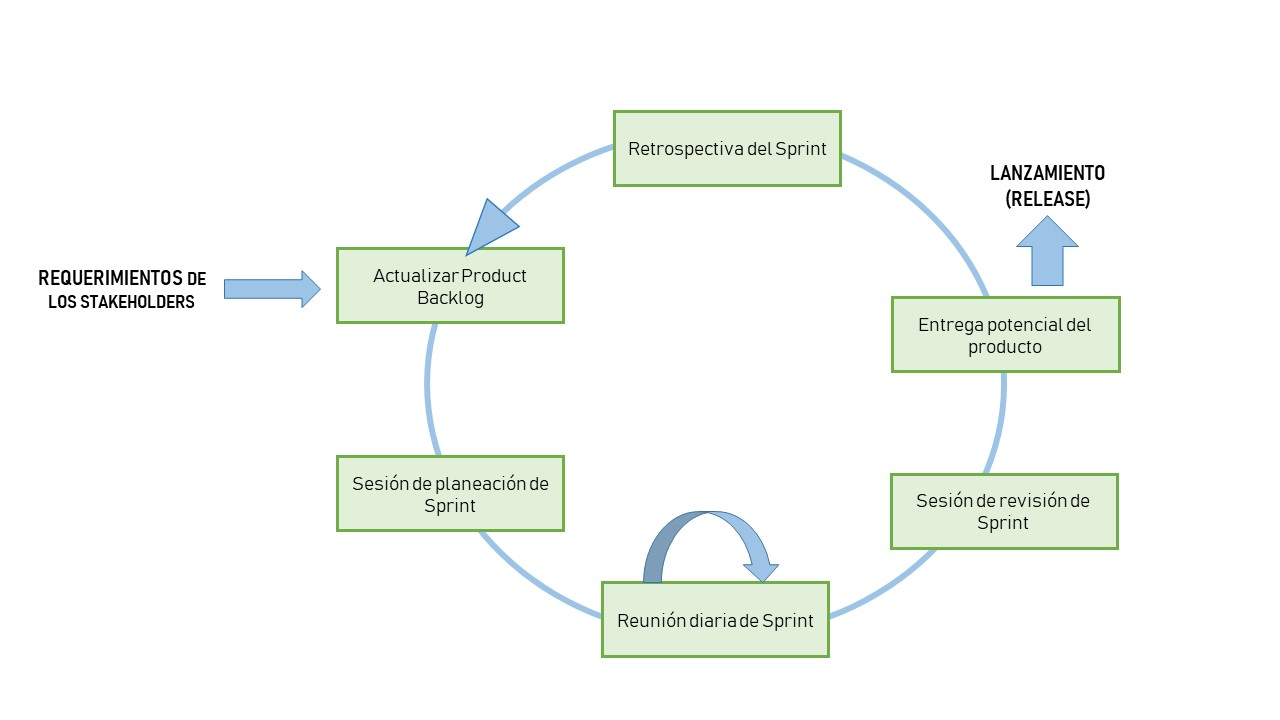
\includegraphics[width=1\textwidth]{Anexos/LATEX/chapters/images/Scrum_1.jpg}
    \caption{Diagrama de Fases y Sprints para el proyecto}
    \small{\textbf{Fuente:} Elaboración propia}
    \label{SCRUM2}
\end{figure}

Con la finalidad de dar soporte a los sprint diarios, se utilizará la plataforma de desarrollo colaborativo Github, facilitando el alojamiento del proyecto y obteniendo control sobre el versionamiento.


